\documentclass[tikz,border=10pt]{standalone}
\usepackage{tikz}
\usetikzlibrary{arrows.meta,calc}

\definecolor{figazul}{RGB}{2,132,199}
\definecolor{figrojo}{RGB}{220,38,38}
\definecolor{figverde}{RGB}{22,163,74}

\begin{document}
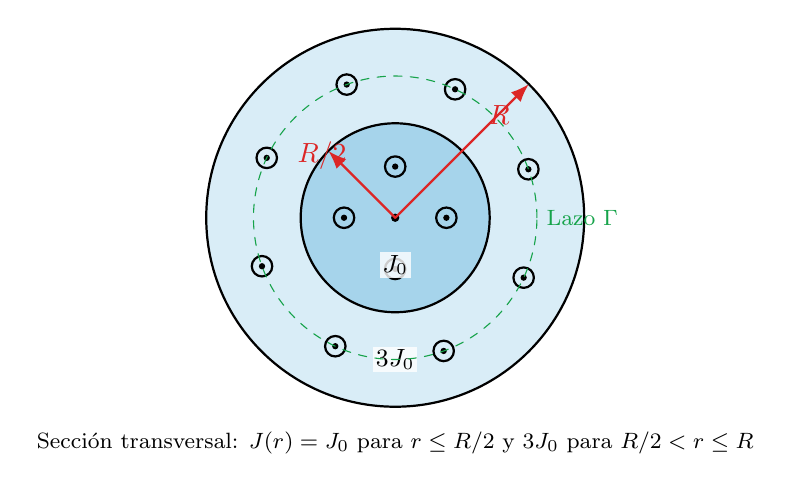
\begin{tikzpicture}[>=Latex, line cap=round, line join=round]
  % Círculo exterior radio R = 2.4
  \draw[thick, fill=figazul!15] (0,0) circle (2.4);

  % Círculo interior radio R/2 = 1.2
  \draw[thick, fill=figazul!35] (0,0) circle (1.2);

  % Centro O
  \fill (0,0) circle (1.5pt);

  % Símbolos de corriente saliente (odot)
  % Zona central (0 <= r <= R/2): J0 (menos densa)
  \foreach \ang in {0, 90, 180, 270} {
    \draw[thick] (\ang:0.65) circle (0.13);
    \fill (\ang:0.65) circle (0.04);
  }

  % Zona exterior (R/2 < r <= R): 3J0 (más densa)
  \foreach \ang in {20, 65, 110, 155, 200, 245, 290, 335} {
    \draw[thick] (\ang:1.8) circle (0.13);
    \fill (\ang:1.8) circle (0.04);
  }

  % Cotas de radio
  % Radio R/2 hacia arriba-izquierda (135°)
  \draw[->, thick, color=figrojo] (0,0) -- (135:1.2);
  \node[above left, color=figrojo] at (135:0.7) {$R/2$};

  % Radio R hacia arriba-derecha (45°)
  \draw[->, thick, color=figrojo] (0,0) -- (45:2.4);
  \node[above right, color=figrojo] at (45:1.5) {$R$};

  % Etiquetas de densidades
  \node[color=black, font=\small, fill=white, fill opacity=0.8, text opacity=1, inner sep=1pt] at (0, -0.6) {$J_0$};
  \node[color=black, font=\small, fill=white, fill opacity=0.8, text opacity=1, inner sep=1pt] at (0, -1.8) {$3J_0$};

  % Lazo amperiano opcional punteado
  \draw[dashed, thin, color=figverde] (0,0) circle (1.8);
  \node[right, font=\footnotesize, color=figverde] at (1.8, 0) {Lazo $\Gamma$};

  % Título / Leyenda inferior
  \node[below, font=\footnotesize] at (0, -2.6) 
    {Sección transversal: $J(r) = J_0$ para $r \le R/2$ y $3J_0$ para $R/2 < r \le R$};
\end{tikzpicture}
\end{document}
